% Copyright 2006 by Till Tantau
%
% This file may be distributed and/or modified
%
% 1. under the LaTeX Project Public License and/or
% 2. under the GNU Free Documentation License.
%
% See the file doc/generic/pgf/licenses/LICENSE for more details.


\section{Fitting Library}
\label{section-library-fit}

\begin{tikzlibrary}{fit}
    The library defines (currently only two) options for fitting a node so that
    it contains a set of coordinates.
\end{tikzlibrary}
%
\begin{codeexample}[setup code,hidden]
    \usetikzlibrary{fit}
\end{codeexample}

When you load this library, the following options become available:

\begin{key}{/tikz/fit=\meta{coordinates or nodes}}
    This option must be given to a |node| path command. The \meta{coordinates
    or nodes} should be a sequence of \tikzname\ coordinates or node names,
    one directly after the other without commas (like with the
    |plot coordinates| path operation). Examples are |(1,0) (2,2)| or
    |(a) (1,0) (b)|, where |a| and |b| are nodes.

    For this sequence of coordinates, a minimal bounding box is computed that
    encompasses all the listed \meta{coordinates or nodes}. For coordinates in
    the list, the bounding box is guaranteed to contain this coordinate, for
    nodes it is guaranteed to contain the |east|, |west|, |north| and |south|
    anchors of the node. In principle (the details will be explained in a
    moment), things are now set up such that the text box of the node will be
    exactly this bounding box.

    Here is an example: We fit several points in a rectangular node. By setting
    the |inner sep| to zero, we see exactly the text box of the node. Then we
    fit these points again in a circular node. Note how the circle encompasses
    exactly the same bounding box.
    %
\begin{codeexample}[]
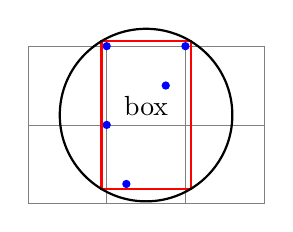
\begin{tikzpicture}[inner sep=0pt,thick,
                    dot/.style={fill=blue,circle,minimum size=3pt}]
  \draw[help lines] (0,0) grid (3,2);
  \node[dot] (a) at (1,1) {};
  \node[dot] (b) at (2,2) {};
  \node[dot] (c) at (1,2) {};
  \node[dot] (d) at (1.25,0.25) {};
  \node[dot] (e) at (1.75,1.5) {};

  \node[draw=red,   fit=(a) (b) (c) (d) (e)] {box};
  \node[draw,circle,fit=(a) (b) (c) (d) (e)] {};
\end{tikzpicture}
\end{codeexample}

    Every time the |fit| option is used, the following style is also applied to
    the node:
    %
    \begin{stylekey}{/tikz/every fit (initially \normalfont empty)}
        Set this style to change the appearance of a node that uses the |fit|
        option.
    \end{stylekey}

    The exact effects of the |fit| option are the following:
    %
    \begin{enumerate}
        \item A minimal bounding box containing all coordinates is computed.
            Note that if a coordinate like |(a)| is used that contains a node
            name, this has the same effect as explicitly providing the
            |(a.north)| and |(a.south)| and |(a.west)| and |(a.east)|. If you
            wish to refer only to the center of the |a| node, use  |(a.center)|
            instead.
        \item The |text width| option is set to the width of this bounding box.
        \item The |align=center| option is set.
        \item The |anchor| is set to |center|.
        \item The |at| position of the node is set to the center of the
            computed bounding box.
        \item After the node has been typeset, its height and depth are
            adjusted such that they add up to the height of the computed
            bounding box and such that the text of the node is vertically
            centered inside the box.
    \end{enumerate}
    %
    The above means that, generally speaking, if the node contains text like
    |box| in the above example, it will be centered inside the box. It will be
    difficult to put the text elsewhere, in particular, changing the |anchor|
    of the node will not have the desired effect. Instead, what you should do
    is to create a node with the |fit| option that does not contain any text,
    give it a name, and then use normal nodes to add text at the desired
    positions. Alternatively, consider using the |label| or |pin| options.

    Suppose, for instance, that in the above example we want the word ``box''
    to appear inside the box, but at its top. This can be achieved as follows:
    %
\begin{codeexample}[]
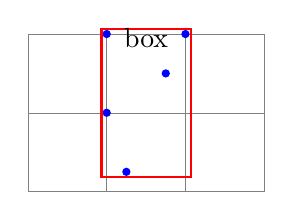
\begin{tikzpicture}[inner sep=0pt,thick,
                    dot/.style={fill=blue,circle,minimum size=3pt}]
  \draw[help lines] (0,0) grid (3,2);
  \node[dot] (a) at (1,1) {};
  \node[dot] (b) at (2,2) {};
  \node[dot] (c) at (1,2) {};
  \node[dot] (d) at (1.25,0.25) {};
  \node[dot] (e) at (1.75,1.5) {};

  \node[draw=red,fit=(a) (b) (c) (d) (e)] (fit) {};
  \node[below] at (fit.north) {box};
\end{tikzpicture}
\end{codeexample}

    Here is a real-life example that uses fitting:
    %
\begin{codeexample}[]
\begin{tikzpicture}
  [vertex/.style={minimum size=2pt,fill,draw,circle},
   open/.style={fill=none},
   sibling distance=1.5cm,level distance=.75cm,
   every fit/.style={ellipse,draw,inner sep=-2pt},
   leaf/.style={label={[name=#1]below:$#1$}},auto]

  \node [vertex] (root) {}
  child { node [vertex,open] {}
    child { node [vertex,open] {}
      child { node [vertex] (b's parent) {}
        child { node [vertex] {}
          child { node [vertex,leaf=d] {} }
          child { node [vertex,leaf=e] {} } }
        child { node [vertex,leaf=b] {} } }
      child { node [vertex,leaf=a] {} } }
    child { node [coordinate] {}
      child[missing]
      child { node [vertex] (f's parent) {}
        child { node [vertex,leaf=c] {} }
        child { node [vertex,leaf=f] {} } } }
    edge from parent node {$\rho$} };

  \node [fit=(d) (e) (b) (b's parent),label=above left:$F^{(b,R)}$] {};
  \node [fit=(c) (f) (f's parent),label=above right:$F^{(c,R)}$]    {};
\end{tikzpicture}
\end{codeexample}
    %
\end{key}

\begin{key}{/tikz/rotate fit=\meta{angle} (initially 0)}
    This key fits \meta{coordinates or nodes} inside a node that is rotated by
    \meta{angle}. As a side effect, it also sets the |/tikz/rotate| key.
    %
\begin{codeexample}[]
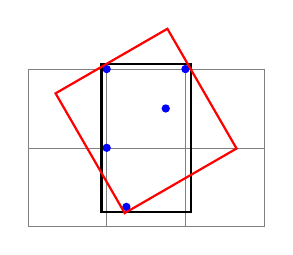
\begin{tikzpicture}[inner sep=0pt,thick,
  dot/.style={fill=blue,circle,minimum size=3pt}]
  \draw[help lines] (0,0) grid (3,2);
  \node[dot] (a) at (1,1) {};
  \node[dot] (b) at (2,2) {};
  \node[dot] (c) at (1,2) {};
  \node[dot] (d) at (1.25,0.25) {};
  \node[dot] (e) at (1.75,1.5) {};
  \node[draw, fit=(a) (b) (c) (d) (e)] {};
  \node[draw=red, rotate fit=30, fit=(a) (b) (c) (d) (e)] {};
\end{tikzpicture}
\end{codeexample}
    %
\end{key}
